% !TEX root = ../../main.tex
% !TeX spellcheck = de_DE

\chapter{Stand der Technik}

\section{General Adversarial Network}
Der Begriff GAN \textit{(General Adversarial Network)} ist auf Ian Goodfellow zurückzuführen \cite{gan-original-paper}.
Das Wort bezeichnet ein Konstrukt aus 2 neuronalen Netzen, die sich gegenseitig trainieren.
Durch das spezielle Training gelingt die Generierung von realistischen unechten Daten.
Solche Daten können dann zum Beispiel für das Training anderer neuronalen Netze \cite{gan-application-augmenting-training-data}, in der Bildverarbeitung \cite{gan-application-upscaling, gan-application-blending} und vielen weiteren Anwendungsgebieten verwendet werden \cite{gan-application-dna-optimizes-protein-functions, gan-application-audio-synthesis}.

\begin{figure}[H]
	\centering
	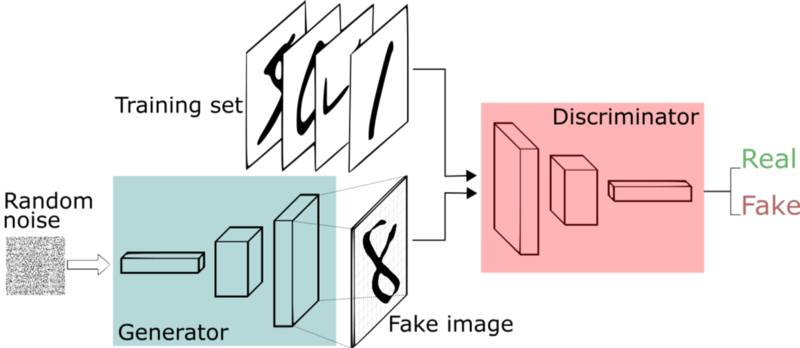
\includegraphics[width=12cm]{kapitel/2_stand_der_technik/img/GAN.png}
	\label{img:gan}
	\caption{Generative Adversarial Network (Bild von Thalles Silva \cite{img-gan})}
\end{figure}

Die beiden Netze eines GANs werden in den Generator und den Discriminator unterschieden.
Aufgabe des Generators ist die Generierung von unechten Daten.
Dafür wandelt er eine zufälligen Eingabe in einen möglichst realistischen Output um.
Die zufällige Eingabe dient dabei als Basis für die Ausgabedaten.
Das ist notwendig, da der Umwandlungsprozess selbst deterministisch ist, aber trotzdem eine Vielzahl an unterschiedlichen Daten generiert werden soll.
\newline

Der Output des Generators wird vom Discriminator klassifiziert.
Dafür wird er sowohl auf die generierten Daten als auch einen Bestand an echten Daten trainiert.
Sein Ziel ist es dann, die falschen Daten des Generators zu identifizieren.
Ziel des Generators hingegen ist es, den Discriminator zu täuschen und die generierten Daten als echt wirken zu lassen.
\newline

Ian Goodfellow bezeichnet den Lernprozess auch als Minimax-Spiel, bei die Ausgabe des Discriminators die zu optimierende Größe ist.
Das bedeutet, der Generator versucht die Genauigkeit des Discriminators zu verringern, während der Discriminator sie erhöhen möchte. \cite{gan-minimax} 
\newline


Für diese Arbeit werden zusätzlich Label eingeführt, um die generierten Daten beeinflussen zu können. 
Diese Art von GAN nennt sich CGAN oder Conditional GAN \cite{gan-conditional}.
Dazu erhalten der Generator und Discriminator das Datenlabel als einen weiteren Input.
So kann der Discriminator aus den echten Daten lernen, dass Daten bei bestimmten Labeln bestimmte Eigenschaften haben.
Dadurch ist dann der Generator gezwungen, diese Eigenschaften zu berücksichtigen, um den Discriminator wieder zu täuschen.

\section{Verfahren zur Bestimmung von Hyperparametern}
\label{chapter:verfahren-bestimmung-hyperparameter}
\todo{Quelle \cite{hyperparameters-search}}

Hyperparameter dienen der Konfiguration des Trainingsprozesses.
Im Gegensatz zu den Parametern neuronaler Netze werden sie durch das Training nicht verändert.
Bei Hyperparametern handelt es sich zum Beispiel um die Lernrate oder Lossfunction \cite{hyperparameters-gan-using-genetic-algorithm}.
Die Bestimmung von Hyperparametern ist wichtig für den Trainingserfolg des Modells und sollte für jeden Datensatz neu bestimmt werden.


Jedoch sind nicht alle Hyperparameter gleichbedeutend für den Trainingserfolg, beispielsweise die Lernrate zählt zu den dominanteren Faktoren \cite{learning-rate-most-important}.
Zusätzlich unterscheiden sich optimale Hyperparameter bei verschiedenen Datensätzen oder Netzarchitekturen.
Für die Suche nach optimalen Hyperparametern gibt es verschieden Verfahren, die im Folgend vorgestellt werden.

\paragraphNewLine{Manuelle Suche}
Zunächst ist es möglich die Hyperparameter manuell festzulegen.
Das ist vor allem bei unwichtigen Hyperparametern sinnvoll, da dort bekannte Standardwerte gesetzt werden können.
Für eine gründliche Suche aller Hyperparameter ist die manuelle Suche allerdings viel zu aufwändig.

\paragraphNewLine{Gridsearch}
Bei der Gridsearch handelt es sich um eine sehr traditionelle Technik und ist gut mit einem Brute-Force Ansatz vergleichbar \cite{hyperparameters-grid-search}.
Dafür werden zunächst die zu untersuchenden Hyperparameter ausgewählt.
Danach erfolgt die Definition eines Suchintervalls inklusive Intervallschritten für jeden Hyperparameter.
Schließlich wird das neuronale Netzwerk für jede Kombination der Hyperparameterwerte trainiert und die Ergebnisse der einzelnen Durchläufe festgehalten.
\newline

Nach dem Training ist es dann möglich, die einzelnen Ergebnisse zu vergleichen.
Dabei können dann Schemata erkannt und Kombinationen aussortiert werden.
Es ist dann möglich die erfolgversprechendsten Netze weiter zu trainieren, oder direkt eine zufriedenstellende Kombination auszuwählen.
\newline

Insgesamt ist Gridsearch sehr simpel zu implementieren, aber auch sehr ressourcenaufwändig.
Der exakte Aufwand hängt dabei stark von der Anzahl der möglichen Kombinationen der Hyperparameterwerte ab.
Weil es sich bei den Kombinationen um ein ein Kreuzprodukt handelt, wächst der Aufwand mit der Anzahl an Werten auch sehr stark an.
Durch die Möglichkeit von Parallelisierung findet die Gridsearch in der Regel bessere Parameter als die sequentielle manuelle Suche in der gleichen Zeit \cite{hyperparameters-random-search}.

\paragraphNewLine{Random Search}
Die Random Search \cite{hyperparameters-random-search} funktioniert ähnlich wie die Gridsearch, nur werden zufällige Werte statt einem festgelegten Werteraster erzeugt (\cref{img:random-search}).
Die zufälligen Werte haben den Vorteil, dass es weniger Werte-Überlagerungen im Vergleich zur den Raster-Kombinationen gibt.
Deswegen kann die zufällige Suche bei gleich vielen Durchläufen ein größeres Spektrum an Ergebnissen abdecken.
Mittels \textit{Automatic Relevance Determination} \cite{automatic-relevance-determination} ist es dann möglich, den Einfluss und Wertebereich der einzelnen Hyperparameter darzustellen.

\begin{figure}[H]
	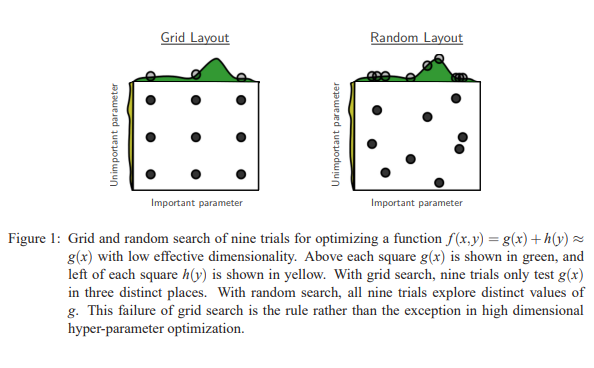
\includegraphics{kapitel/2_stand_der_technik/img/random-vs-grid-search.png}
	\caption{Random Search vs Grid Search (Quelle \cite{hyperparameters-random-search})}
	\label{img:random-search}
\end{figure}

Problem der Random Search ist vor allem, dass die Räume der guten Hyperparameter (\textit{Search Space}) sehr klein sind.
Dadurch ist nicht gewährleistet, dass ein zufälliger Wert auch den Raum trifft.
Jedoch erzielen Optimierungen mittels Random Search in der Regel trotzdem (sehr) gute Ergebnisse.
Dem Grid-Search-Verfahren ist die Random-Search allerdings nicht prinzipiell überlegen \cite{hyperparameters-random-search}.

\paragraphNewLine{Genetic Algorithm - Evolutionäre Suche}
\todo[inline,shadow]{mehr belegen}
Das evolutionäre Suchverfahren wandelt die Hyperparametersuche in einen evolutinären Entwicklungsprozess um.
Die 'Evolution' des Algorithmus ist eine Anlehnung an die natürliche Entwicklung in der Natur.
Diese Entwicklung zeichnet sich durch die Operatoren Selektion, Kombination und Mutation aus, die auch der Algorithmus verwendet. \cite{hyperparameters-search-comparison-focus-genetic, hyperparameters-genetic-algorithm}
\newline

Für den Optimierungsprozess werden am Anfang mehrere zufällige Hyperparameterinstanzen erzeugt.
Die Instanzen werden dann trainiert und stehen im Wettbewerb um das beste Ergebnis.
Nach der Auswertung der Trainingsergebnisse werden die besten Instanzen selektiert und miteinander gekreuzt und oder mutiert.
\newline

Die evolutionäre Suche eignet sich besonders gut bei sehr vielen Hyperparametern.
Im Gegensatz zur Grid-Search werden nicht immer alle Kombinationen ausprobiert, sondern nur einzelne, die sich bereits zuvor als vielversprechend herausgestellt haben.
Dadurch kann mit sehr großen Mengen an Hyperparametern umgegangen werden.

Allerdings ist die evolutionäre Suche vergleichsweise langsam, da die Evolutionsschritte sequentiell ablaufen müssen.
Erst bei einer hohen Anzahl an Hyperparametern oder einem sehr großen Suchraum wird die Grid-Search dann so langsam, dass sich die evolutionäre Suche lohnt \cite{hyperparameters-search-comparison-focus-genetic}.

\section{Related Work}
\label{chapter:related-work}
Es gibt viele verschiedene Versuche und Varianten die Hyperparameter zu optimieren.
Dementsprechend viele Papers und Artikel befassen sich damit.
Einige dieser Arbeiten werden nachfolgend kurz vorgestellt.
\newline

\paragraphNewLine{Best Selection of Generative Adversarial Networks Hyper-Parameters Using Genetic Algorithm \cite{hyperparameters-genetic-algorithm}}
Die Studie befasst sich mit Hyperparameter Optimierung auf Basis von genetischen Algorithmen.
Genetische Algorithmen zeichnen sich unter anderem durch die verwendeten Operatoren Mutation, Kreuzung und Selektion aus \cite{genetic-algorithms}.
Ziel der Studie war es, bestmögliche Hyperparameter für das MNIST Datenset zu finden \cite{dataset:mnist}.
Dabei wurden die Hyperparameter \textit{learning-rate, dropout, batch-size und number of neurons in dense layer} betrachtet.
\newline

Zwar sind die Daten und die Herangehensweise nicht die selbe wie in dieser Arbeit, aber die untersuchten Hyperparameter.
Diese können mit als Basis für die Untersuchung genommen werden.
Zudem verdeutlicht die Arbeit noch einmal die große Auswirkung von Hyperparametern.

\paragraphNewLine{Unsupervised Representation Learning With Deep Convolutional Generative Adversarial Networks \cite{hyperparameters-convolutional-gan}}
Ziel dieser Studie ist es allgemein gute Hyperparameter zu finden.
Dafür wurden Bilder aus verschiedenen Datensets genommen (Large Scale Scene Understanding \cite{dataset:lsun}, Imagenet-1k \cite{dataset:image-net} und einem eigenen Datenset mit Gesichtern).
Bei den Hyperparametern wurden diverse untersucht, zum Beispiel aber nicht ausschließlich die Lernrate, Momentum und Batch-Size.
Im Ergebnis konnten für alle Werte gefunden werden, die über alle Datensets meistens stabil mit zufriedenstellenden Ergebnissen liefen.
\todo{Hyperparameter: learning-rate 0.0002, momentum (beta1) zu 0.5, mini-batch size 128,... (Kapitel 4 Details of adversarial training)}
Erkenntnis der Studie war auch, dass keine Hyperparameter Kombination gefunden werden konnte, die über alle Datensets 100\% stabil laufen konnte.
\newline

Eine allgemeine Studie zum Thema Hyperparameter ist für die Arbeit sehr interessant, da sie gute Ausgangswerte bietet.
Dass keine 100\% stabile Zusammenstellung gefunden werden konnte, verdeutlicht die Notwendigkeit der Feinanpassung an jedes Datenset.


\paragraphNewLine{The GAN Landscape: Losses, Architectures, Regularization, And Normalization \cite{gan-landscape-losses-architectures-regularization-normalization}}
Dieses Studie beschäftigt sich nicht ausschließlich mit Hyperparametertuning.
Aber auch in dieser Studie werden allgemein GANs optimiert und die Erkenntnisse daraus können verwendet werden.
In the GAN Landscape wird das GAN auf die Datensets CIFAR10 \cite{dataset:cifar10}, CELEBA-HQ-128 und LSUN-BEDROOM \cite{dataset:lsun}.
Für das Training wurden dann ein DCGAN und ResNet verglichen.
Dabei fand die Studie viele interssante Erkenntnisse heraus, zum Beispiel eine gute Updatequote von 5:1 zwischen Discriminator und Generator.
\newline

Besonders interessant bei dieser Arbeit ist die Bestimmung von anderen Methoden, wie das unterschiedliche Updaten von Discrimintaor und Generator.
Wieder bietet die Arbeit eine gute Ausgangslage, aber keine Lösung für ein Datenset mit geometrischen Bildern.

\paragraphNewLine{Tunability: Importance of Hyperparameters of Machine Learning Algorithms}
\url{https://www.jmlr.org/papers/volume20/18-444/18-444.pdf}

\begin{comment}
	
\paragraph{Links}
\begin{itemize}
	\item Inception Score zum Rating von erzeugten Bildern (Salimans et al. 2016)
	\item Frechet Inception Distance (Heusel et al. 2017)
	\item stackoverflow \url{https://stackoverflow.com/questions/46386948/adjusting-gan-hyperparameters}
	\item \url{https://openreview.net/pdf?id=rkGG6s0qKQ}
	\item \url{https://arxiv.org/pdf/1511.06434.pdf%C3%AF%C2%BC%E2%80%B0}
	\item Forget the Learning Rate, Decay Loss \url{https://arxiv.org/ftp/arxiv/papers/1905/1905.00094.pdf}
	\item beste learningRate/Dropout/BatchSize/NumberOfNeuronsInDenseLayer mit evolutionären neuronalen netz für mnist 
	\item zum orientieren ?? \cite{gan-conditional}
\end{itemize}


\end{comment}